\documentclass[12pt, aspectratio=1610]{beamer}


\usepackage{beamerSFU-VKR}
\usetikzlibrary{fit,shapes,backgrounds,hobby,arrows.meta,decorations,decorations.pathreplacing,shapes.callouts}
\institute[ИМиФИ СФУ]{ФГАОУ ВО <<Сибирский федеральный университет>>\\
    Институт математики  и фундаментальной информатики\\
	Кафедра высшей и прикладной математики  \\                                  
}
%\direction{Магистерская программа 01.04.02.01 Математическое моделирование}
\title[Маршрутизация на пределе]{Маршрутизация на пределе: живые графы, мертвые дороги и киберпространство}
\author[Солдатенко А. А.]{Солдатенко Александр Александрович}
	


\date[\today]{Красноярск\\\the\year{}}

\renewcommand*{\thefootnote}{\arabic{footnote}}
\setcounter{footnote}{0}

\begin{document}

\begin{frame}[t]
\titlepage
\end{frame}
\section{Введение}

\begin{frame}
\begin{tikzpicture}
	\node[text width=2cm] (a) {\reflectbox{
\includegraphics[width=\textwidth]{Pics/Tourist.png}}};
	\node[text width=2cm,right=of a] {
\includegraphics[width=\textwidth]{Pics/water-fountain.png}};
	\node[text width=2cm, above right=.75cm and 1.5cm of a] (b) {
\includegraphics[width=\textwidth]{Pics/clock-tower.png}};
	\node[text width=2cm, below right=.25cm and 1.25cm of a] (c) {
\includegraphics[width=\textwidth]{Pics/moai.png}};
	\node[text width=2cm, above right=.5cm and .5cm of c] (d) {
\includegraphics[width=\textwidth]{Pics/observatory.png}};
	\node[text width=2cm, above right=.6cm and .25cm of d] (e) {
\includegraphics[width=\textwidth]{Pics/mayan-pyramid.png}};
	\node[text width=2cm, below right=.3cm and .35cm of d] (f) {
\includegraphics[width=\textwidth]{Pics/hobbit-dwelling.png}};
	\node[text width=2cm, below right=.23cm and .35cm of e] (g) {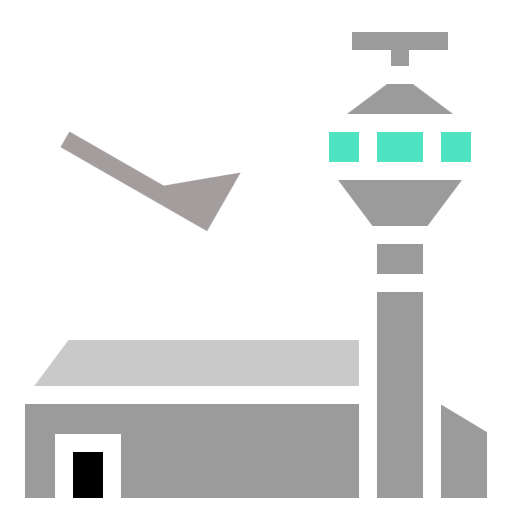
\includegraphics[width=\textwidth]{Pics/control-tower.png}};
\end{tikzpicture}
\end{frame}

\begin{frame}
\frametitle{Абстракция}
\begin{tikzpicture}
	
	\node[text width=7cm] (a) {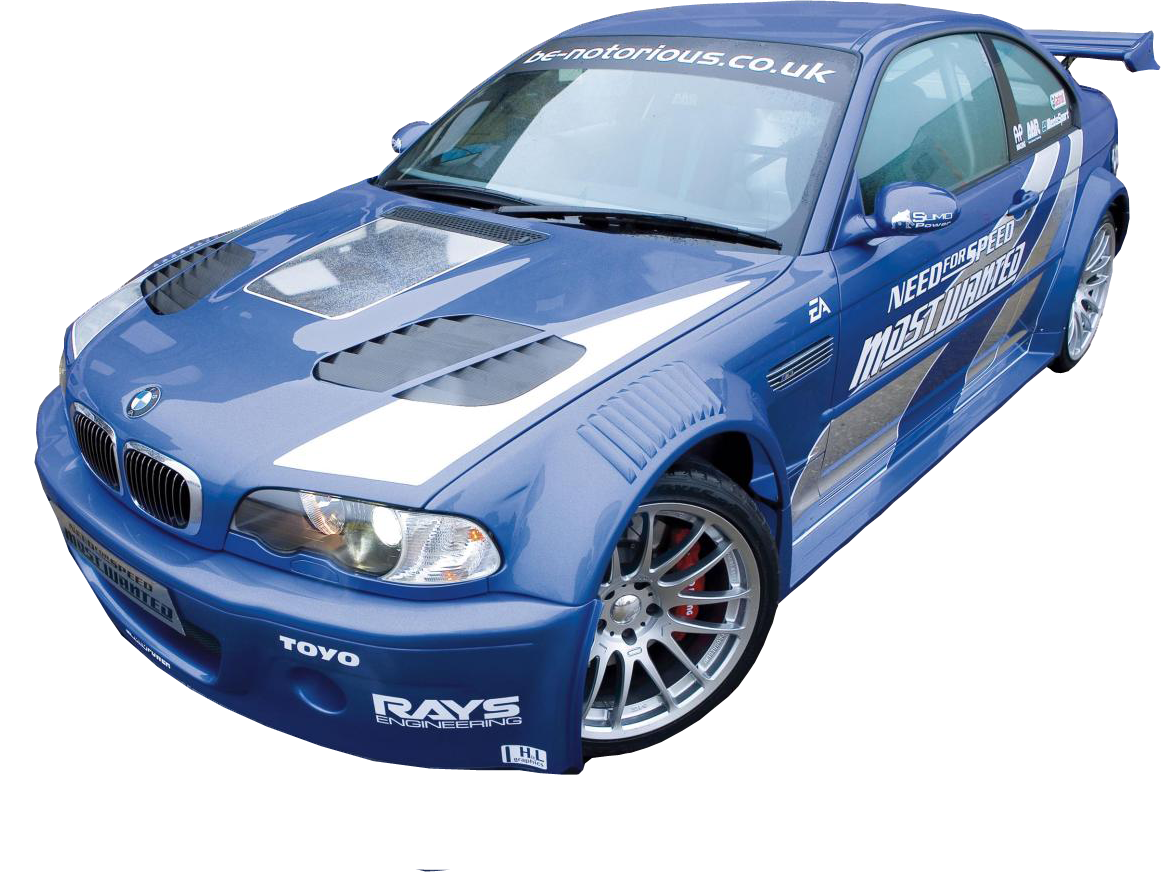
\includegraphics[width=\textwidth]{Pics/beamer.png}};
	\pause
	\node[text width=2cm,left=.25cm of a] (b) {
\includegraphics[width=\textwidth]{Pics/petcat.png}};
	\pause
	\node[text width=2cm,right=.25cm of a] (c) {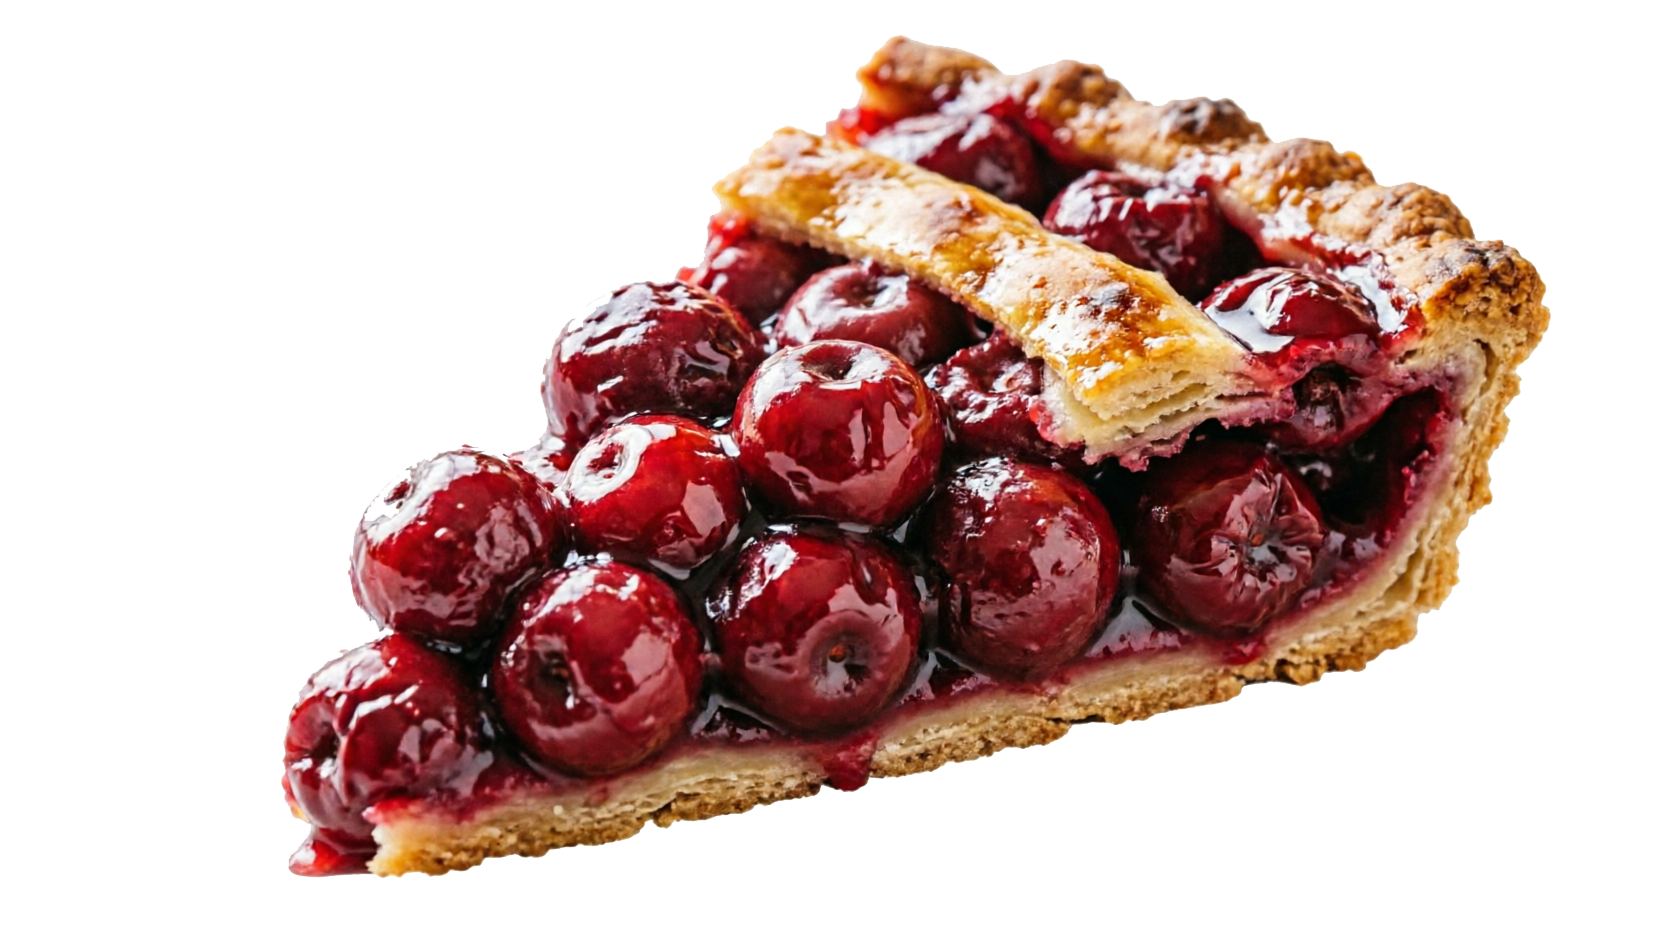
\includegraphics[width=\textwidth]{Pics/cherrypie.png}};
	\node[text width=3cm,above right=-1cm and -1cm of c] (d) {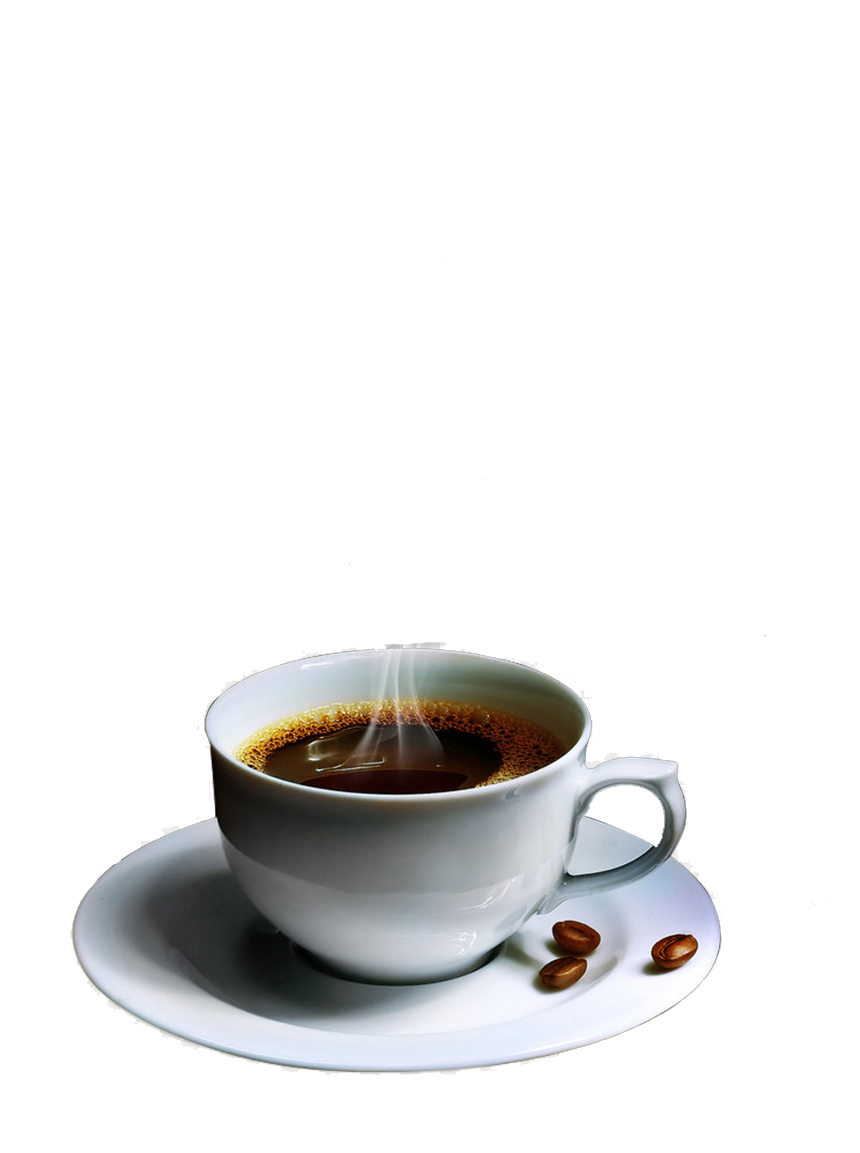
\includegraphics[width=\textwidth]{Pics/coffee.png}};
\end{tikzpicture}
\end{frame}
\section{Кратчайший путь}
\begin{frame}
\frametitle{Формализуем наше путешествие}
\begin{block}{Определения}
	\begin{itemize}
		\item $V$ -- множество вершин, при этом $|V|=n$;
		\item $E$ -- множество ребер, как подмножество $V\times V$, при этом $|E|=m$;
		\item $G=(V,E)$ -- граф c вершинами $V$ и ребрами $E$;
		\item Весовая функция $w(e)\colon E\rightarrow \mathbb{R}$, где $e=(u,v)\in E$ и $u,v\in V$;
		\item Путь $P$ -- последовательность вершин $\{s=v_1,v_2,\dots, v_{n-1},d=v_{n}\}$, 
		
		\hfill где $(v_i,v_{i+1})\in E$ и $v_i\neq v_{i+1}$;
		\item Вес пути $w(P)$ -- сумма всех ребер входящих в путь $\sum\limits_{e=(u,v)\in P}w(e)$.
	\end{itemize}
\end{block}
\begin{center}
	\begin{columns}
		\column{.5\textwidth}
		\begin{tikzpicture}[dnode/.style={draw,circle},node distance = .5cm]
		\node[dnode] (a) {1};
		\node[dnode,above right=0.5cm and 3cm of a] (b) {2};
		\node[dnode,below right=0.5cm and 3cm of a] (c) {3};
		\node[dnode,above right=0.5cm and 3cm of c] (d) {4};
		\draw[-Latex] (a) -- (b) node [above,midway, sloped] {$2$};
		\draw[-Latex] (a) -- (c) node [below,midway, sloped] {$5$};
		\draw[-Latex] (b) -- (d) node [above,midway, sloped] {$3$};
		\draw[-Latex] (c) -- (d) node [below,midway, sloped] {$4$};
\end{tikzpicture}	
\hfill
		\column{.4\textwidth}
			$P_1=\{1,2,4\}, w(P_1)=2+3=5;$

			$P_2=\{1,3,4\}, w(P_2)=5+4=9.$
	\end{columns}

\end{center}
\end{frame}

\begin{frame}
	\frametitle{Формализуем наше путешествие}
	\begin{block}{Задача о кратчайшем пути}
		\begin{tabular}{>{\bfseries}rp{.8\textwidth}}
			Дано: & граф $G=(V,E)$, весовая функция $w(e)$, стартовая вершина $s$ и целевая вершина $d$.\\
			Требуется: & найти кратчайший путь $P$ и последовательность образующих его вершин.
		\end{tabular}
	\end{block}
	Под кратчайшим путем понимается такой путь $P=\arg\min\limits_{P}\big\{w(P)\colon s\mathrel{\leadsto}d\big\}$.

	Для удобства ещё определим функцию $dist(s,d)$, которая обозначает вес кратчайшего пути $P$ от вершины $s$ до вершины $d$.
\end{frame}

\begin{frame}
	\frametitle{Как найти кратчайший путь}
	\hspace*{-.25cm}
	\begin{tabular}{p{.49\textwidth}p{.49\textwidth}}
		
		{\bfseries Алгоритм Дейкстры} & {\bfseries Алгоритм Беллмана-Форда}\\

		Последовательно перебирает все окрестные вершины, пока не выберет  целевую вершину в качестве активной. & Последовательно релаксирует по всем ребрам для каждой длины пути, в итоге получает матрицу с кратчайшими весами от $s$ до всех остальных вершин.\\
		\begin{itemize}
			\item[$+$] Работает быстро $\mathcal{O}(n\log m)$
			\item[$-$] Не работает с отрицательными весами
		\end{itemize}
		&
		\begin{itemize}
			\item[$+$] Работает с отрицательными весами
			\item[$-$] Работает медленнее  $\mathcal{O}(n\cdot m)$
		\end{itemize}\\
	\end{tabular}

\end{frame}

\begin{frame}
	\centering
	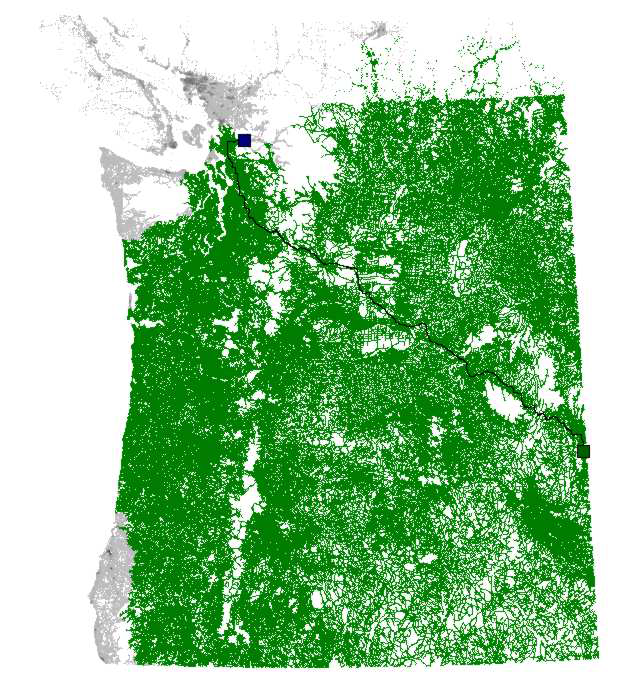
\includegraphics[height = \paperheight]{Pics/Di.png}
\end{frame}

\begin{frame}
	\frametitle{Как можно сделать это быстрее?}
	\begin{overprint}
		\onslide<1>
		\begin{tikzpicture}
	\node[text width=2cm] (a) {\reflectbox{
\includegraphics[width=\textwidth]{Pics/Tourist.png}}};
	\node[draw, cloud callout, cloud puffs=15, aspect=2.5, cloud puff arc=120,text width = 3cm,anchor = pointer,above left=.5 and -1.5 of a,align=center] {Зачем мне эти графы? Я же вижу цель!};	
	\node[text width=4cm,above right=.25 and 4 of a] {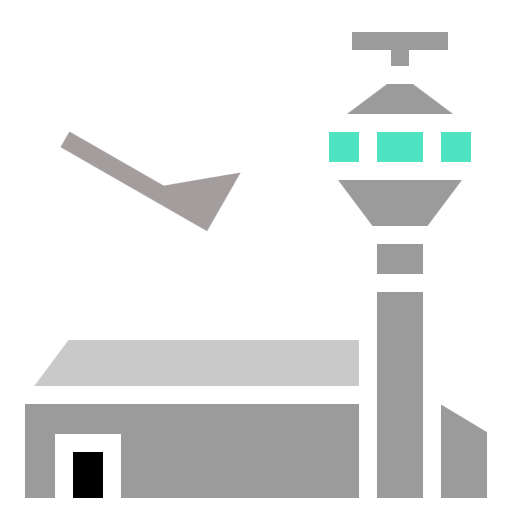
\includegraphics[width=\textwidth]{Pics/control-tower.png}};
	\end{tikzpicture}
	\onslide<2>
	\begin{tikzpicture}
	\node[text width=2cm] (a) {\reflectbox{
\includegraphics[width=\textwidth]{Pics/Tourist.png}}};
	\node[draw, cloud callout, cloud puffs=15, aspect=2.5, cloud puff arc=120,text width = 3cm,anchor = pointer,above left=.5 and -1.5 of a,align=center] {Чёрт!};	
	\node[text width=4cm,above right=.25 and 4 of a] {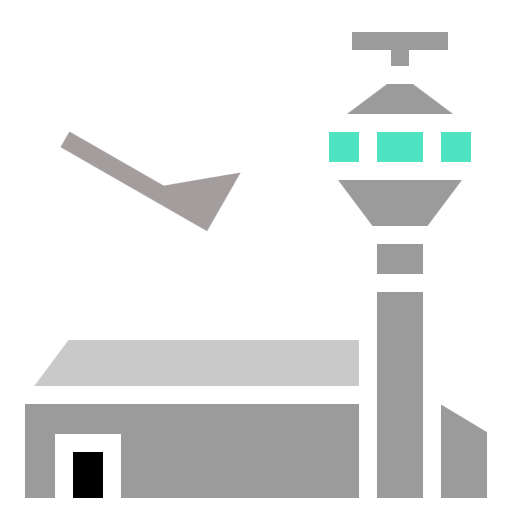
\includegraphics[width=\textwidth]{Pics/control-tower.png}};
	\node[text width = 7cm, right=of a] {\reflectbox{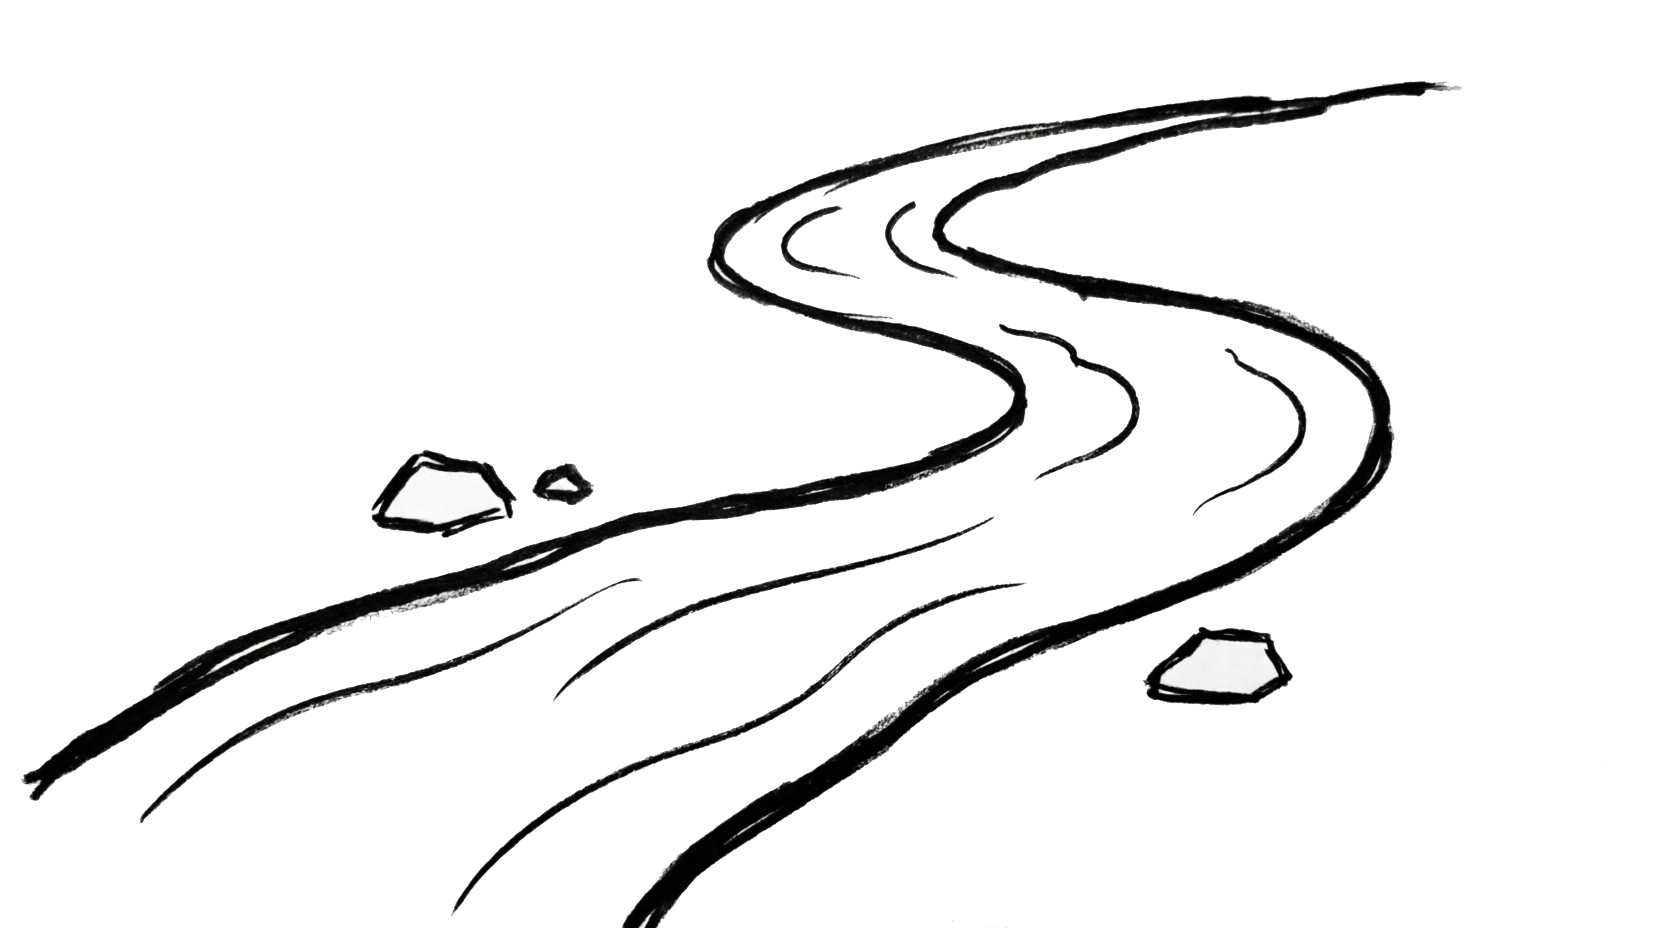
\includegraphics[width=\textwidth]{Pics/river.png}}};
	\end{tikzpicture}
	\end{overprint}
	
\end{frame}

\begin{frame}
	\frametitle{Как можно сделать это быстрее?}
	Введем некоторую функцию $\pi(v)$, которая оценивая оставшийся путь от $v$ до $d$. Функция $\pi(v)$ называется потенциальной если удовлетворяет двум свойствам.
	\begin{block}{Свойства потенциальной функции}
		\begin{itemize}
			\item \textbf{Допустимость} $$\pi(v) \leq dist(v,d);$$
			\item \textbf{Преемственность} $$\pi(v)\leq dist(v,u) + \pi(u).$$
		\end{itemize}
	\end{block}
	\vspace*{-1cm}
	\begin{center}
		\begin{tikzpicture}
		\node[text width = 5cm] {\includegraphics[width=\textwidth]{Pics/map.png}};
		\node[text width = 3cm,rotate=30] {
\includegraphics[width=\textwidth]{Pics/rule.png}};
		\end{tikzpicture}
	\end{center}
	
\end{frame}

\begin{frame}
	\frametitle{Ещё быстрее?!}
	\centering
	\begin{tikzpicture}[node distance = .1]
		\node[text width = 2cm] (a) {\reflectbox{
\includegraphics[width=\textwidth]{Pics/Tourist.png}}};
		\node[text width = 10cm,right=of a] (b) {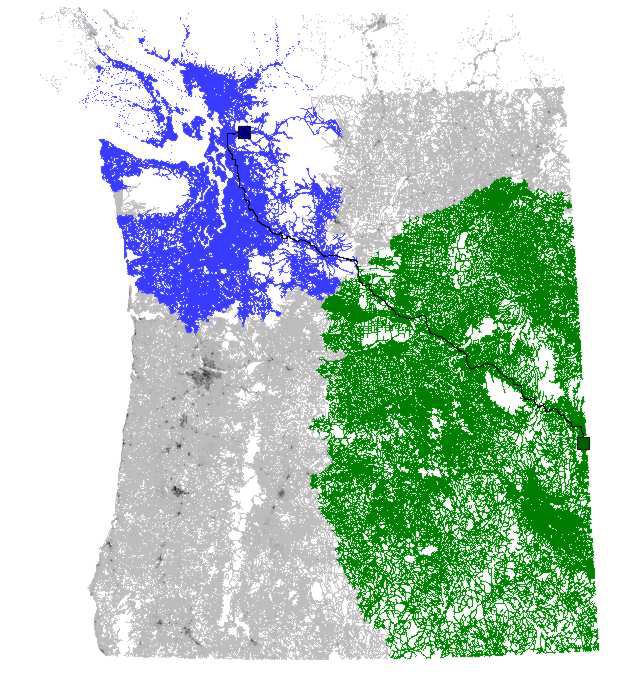
\includegraphics[height=\paperheight]{Pics/Bi.png}};
		\node[text width = 2cm,right=of b] (c) {
\includegraphics[width=\textwidth]{Pics/Tourist.png}};
	\end{tikzpicture}
\end{frame}

\begin{frame}
	\frametitle{Ещё быстрее?!}
	\begin{overprint}
		\onslide<1>
		\begin{center}
			\begin{tikzpicture}[node distance = .5]
		\node (a) {Предобработка};
		\node[below left=of a] (land) {Ориентиры};
		\node[below=of a] (hier) {Иерархия};
		\node[below right=of a] (mark) {Маркировка};
		\draw[->] (a) -- (land);
		\draw[->] (a) -- (hier);
		\draw[->] (a) -- (mark);
	\end{tikzpicture}
		\end{center}
		
	\onslide<2>
	\begin{center}
			\begin{tikzpicture}[node distance = .5]
		\node (a) {Предобработка};
		\node[below left=of a,draw,red] (land) {Ориентиры};
		\node[below=of a] (hier) {Иерархия};
		\node[below right=of a] (mark) {Маркировка};
		\draw[->] (a) -- (land);
		\draw[->] (a) -- (hier);
		\draw[->] (a) -- (mark);
	\end{tikzpicture}
	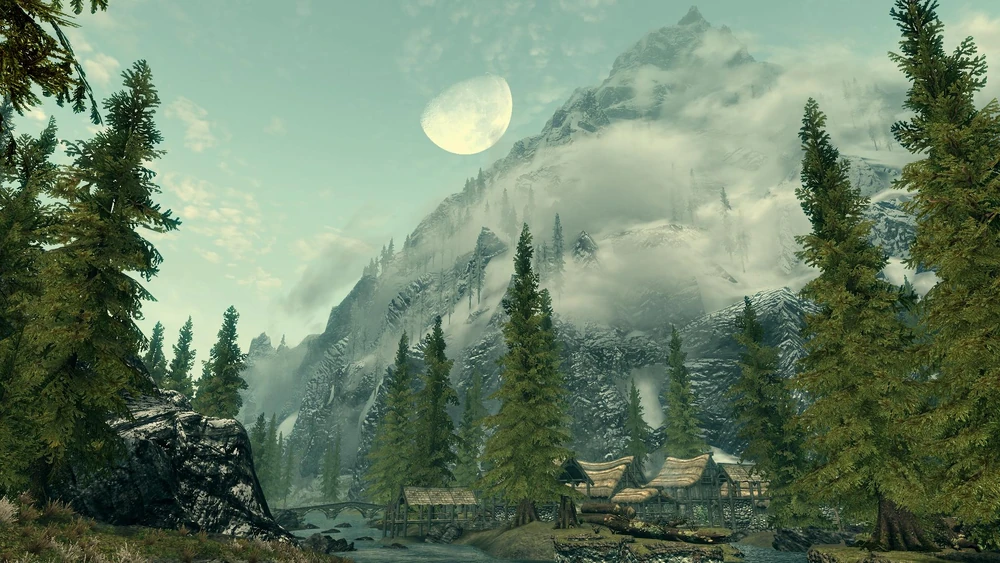
\includegraphics[height = .5\paperheight]{Pics/mountain.png}
		\end{center}

	
	\onslide<3>
	\begin{center}
			\begin{tikzpicture}[node distance = .5]
		\node (a) {Предобработка};
		\node[below left=of a,draw,red] (land) {Ориентиры};
		\node[below=of a] (hier) {Иерархия};
		\node[below right=of a] (mark) {Маркировка};
		\draw[->] (a) -- (land);
		\draw[->] (a) -- (hier);
		\draw[->] (a) -- (mark);
	\end{tikzpicture}
	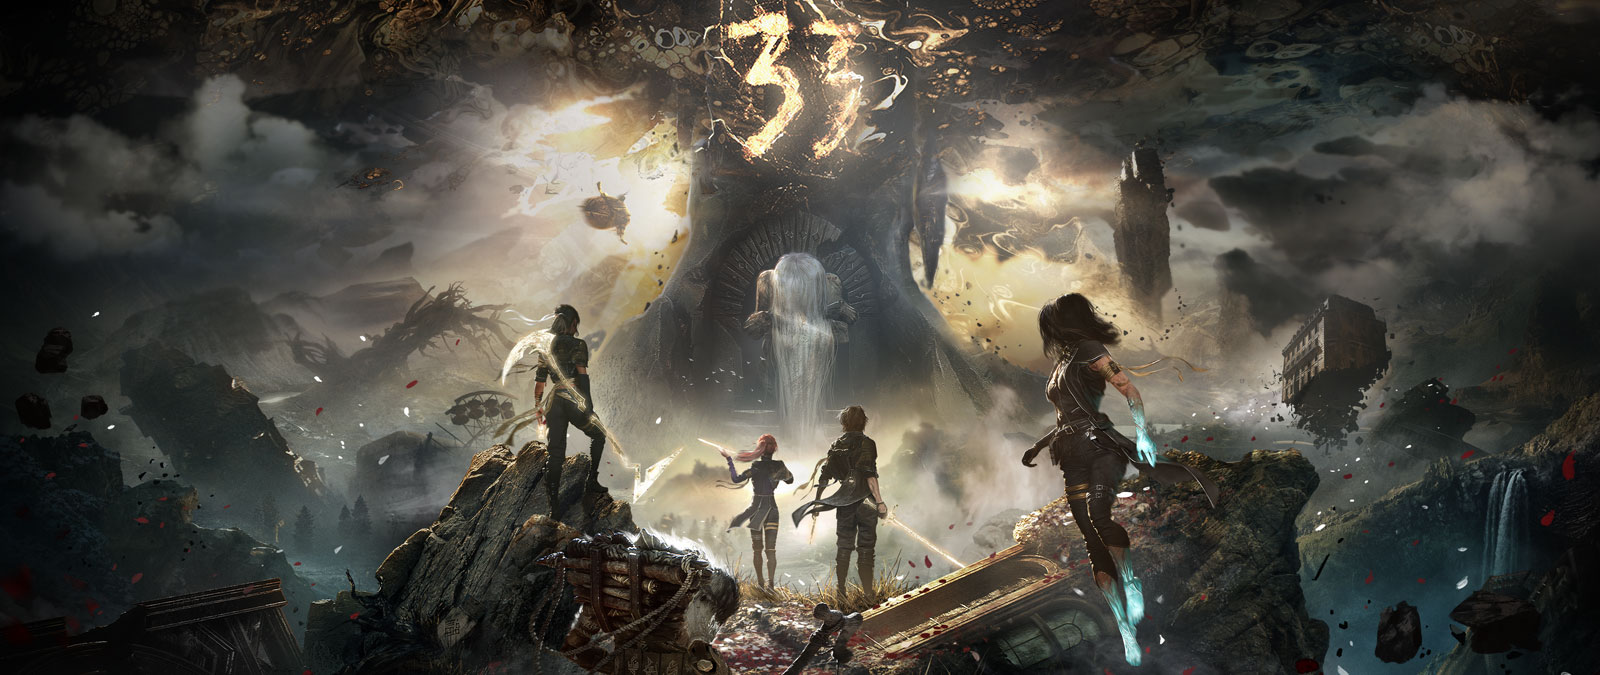
\includegraphics[height = .5\paperheight,clip,trim=100 0 100 0]{Pics/expedition.jpg}
		\end{center}
	
	\onslide<4>
	\begin{center}
			\begin{tikzpicture}[node distance = .5]
		\node (a) {Предобработка};
		\node[below left=of a] (land) {Ориентиры};
		\node[below=of a,draw,red] (hier) {Иерархия};
		\node[below right=of a] (mark) {Маркировка};
		\draw[->] (a) -- (land);
		\draw[->] (a) -- (hier);
		\draw[->] (a) -- (mark);
	\end{tikzpicture}
	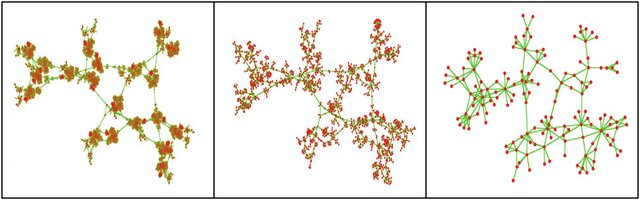
\includegraphics[height = .4\paperheight]{Pics/hier.jpg}
		\end{center}
	\onslide<5>
	\begin{center}
			\begin{tikzpicture}[node distance = .5]
		\node (a) {Предобработка};
		\node[below left=of a] (land) {Ориентиры};
		\node[below=of a] (hier) {Иерархия};
		\node[below right=of a,draw,red] (mark) {Маркировка};
		\draw[->] (a) -- (land);
		\draw[->] (a) -- (hier);
		\draw[->] (a) -- (mark);
	\end{tikzpicture}
	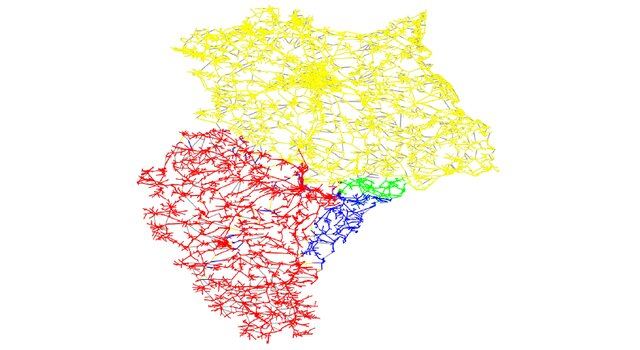
\includegraphics[height = .5\paperheight]{Pics/arc.jpg}
		\end{center}
	\end{overprint}
	
\end{frame}

\section{Живые графы}

\begin{frame}
	\frametitle{Обстановка изменчива}
\begin{columns}
	\column{.5\textwidth}
	
\includegraphics[width=\textwidth]{Pics/Asphalt.png}
	\pause
	\column{.5\textwidth}
	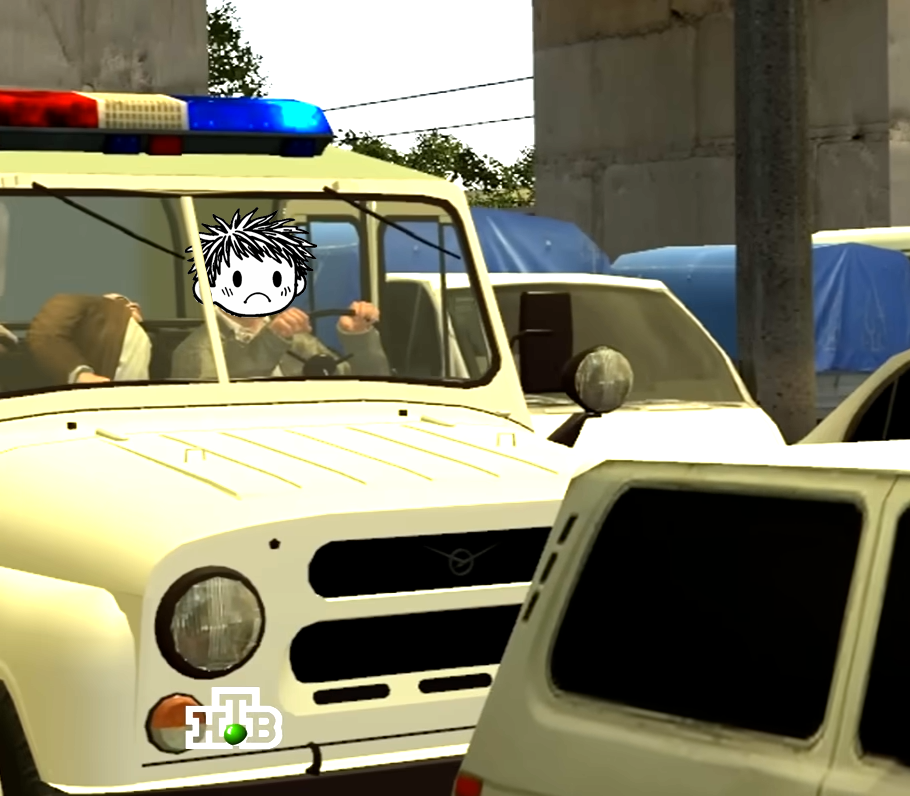
\includegraphics[width=\textwidth]{Pics/Jam.png}
\end{columns}
\end{frame}

\begin{frame}
	\frametitle{Обстановка изменчива}
	\begin{block}{Определения}
		\begin{itemize}
			\item Величина $t>0$, измеряется в условных единицах времени и принимает значения из некоторого конечного множества $T$;
			\item Весовая функция $w_{xy}(t)\geq 0$, зависящая от времени $t$, для ребра $(x,y)\in E$;
			\item Функция прибытия $F_{xy}(t) = t+w_{xy}(t)$, где
			
			\qquad $t$ -- время отправления из $x$, 
			
			\qquad $F_{xy}(t)$ -- время прибытия в вершину $y$.
		\end{itemize}
	\end{block}
	\pause
	\begin{block}{Условие FIFO}
		Если для любых моментов времени $0\leq t_1\leq t_2$ выполняется неравенство $$F_{xy}(t_1)\leq F_{xy}(t_2),$$ то говорят, что функция прибытия для ребра $(x,y)\in E$ является монотонной.
	\end{block}
\end{frame}

\begin{frame}
	\frametitle{Обстановка изменчива}
	\begin{overprint}
		
	
	\onslide<1>
	\begin{tikzpicture}
      \begin{axis}
        [
          axis lines = center,
          every axis y label/.style={at={(ticklabel cs:0.5)},rotate=90,anchor=center,},
          every axis x label/.style={at={(ticklabel cs:0.5)},anchor=center,},
          height=5cm,
          width=15cm,
          xlabel={Время отправления, часы},
          ylabel={Время в пути, мин.},
          xmin=0, xmax=24,
          ymin=0, ymax=3,
          xtick=data,
          xticklabel style={rotate=45, anchor=east},
          xticklabels={,$7{:}00$,$8{:}00$,$9{:}00$,$17{:}00$,$18{:}00$,$19{:}00$,$22{:}00$,$24{:}00$},
          yticklabels={,$0$,$30$,$60$,$90$},
        ]
        \addplot coordinates
        {
          (0,1)
          (7,1)
          (8,3)
          (9,2)
          (17,2)
          (18,3)
          (19,2)
          (22,2)
          (24,1)
        };
      \end{axis}
    \end{tikzpicture}
	\onslide<2>
	\begin{tikzpicture}%[scale=0.5]
      \begin{axis}
        [
          axis lines = center,
          every axis y label/.style={at={(ticklabel cs:0.5)},rotate=90,anchor=center,},
          every axis x label/.style={at={(ticklabel cs:0.5)},anchor=center,},
          height=5cm,
          width=15cm,
          xlabel={Время отправления, часы},
          ylabel={Время в пути, мин.},
          xmin=0, xmax=24,
          ymin=0, ymax=3,
          xtick=data,
          xticklabel style={rotate=45, anchor=east},
          xticklabels={,$7{:}00$,$8{:}00$,$9{:}00$,$17{:}00$,$18{:}00$,$19{:}00$,$22{:}00$,$24{:}00$},
          yticklabels={,$0$,$30$,$60$,$90$},
        ]
        \addplot coordinates
        {
          (0,1)
          (7,1)
          (8,3)
          (9,3)
          (17,3)
          (18,3)
          (19,3)
          (22,2)
          (24,1)
        };
      \end{axis}
    \end{tikzpicture}
	\end{overprint}
\end{frame}

\begin{frame}
	\frametitle{Решение есть}
	\begin{block}{Задача Time-Dependend Shortest Path}
		\begin{tabular}{>{\bfseries}rp{.8\textwidth}}
			Дано: & нестационарный граф $G=(V,E)$, весовая функция $w_{xy}(t)$, удовлетворяющая условию FIFO, стартовая вершина $s$ и целевая вершина~$d$.\\
			Требуется: & найти кратчайший путь $P$ и последовательность образующих его вершин.
		\end{tabular}
	\end{block}
	Алгоритм Дейкстры с небольшой доработкой способен решать задачу TDSP.
	
\end{frame}

\begin{frame}
	\frametitle{Обстановка накаляется}
	\centering
	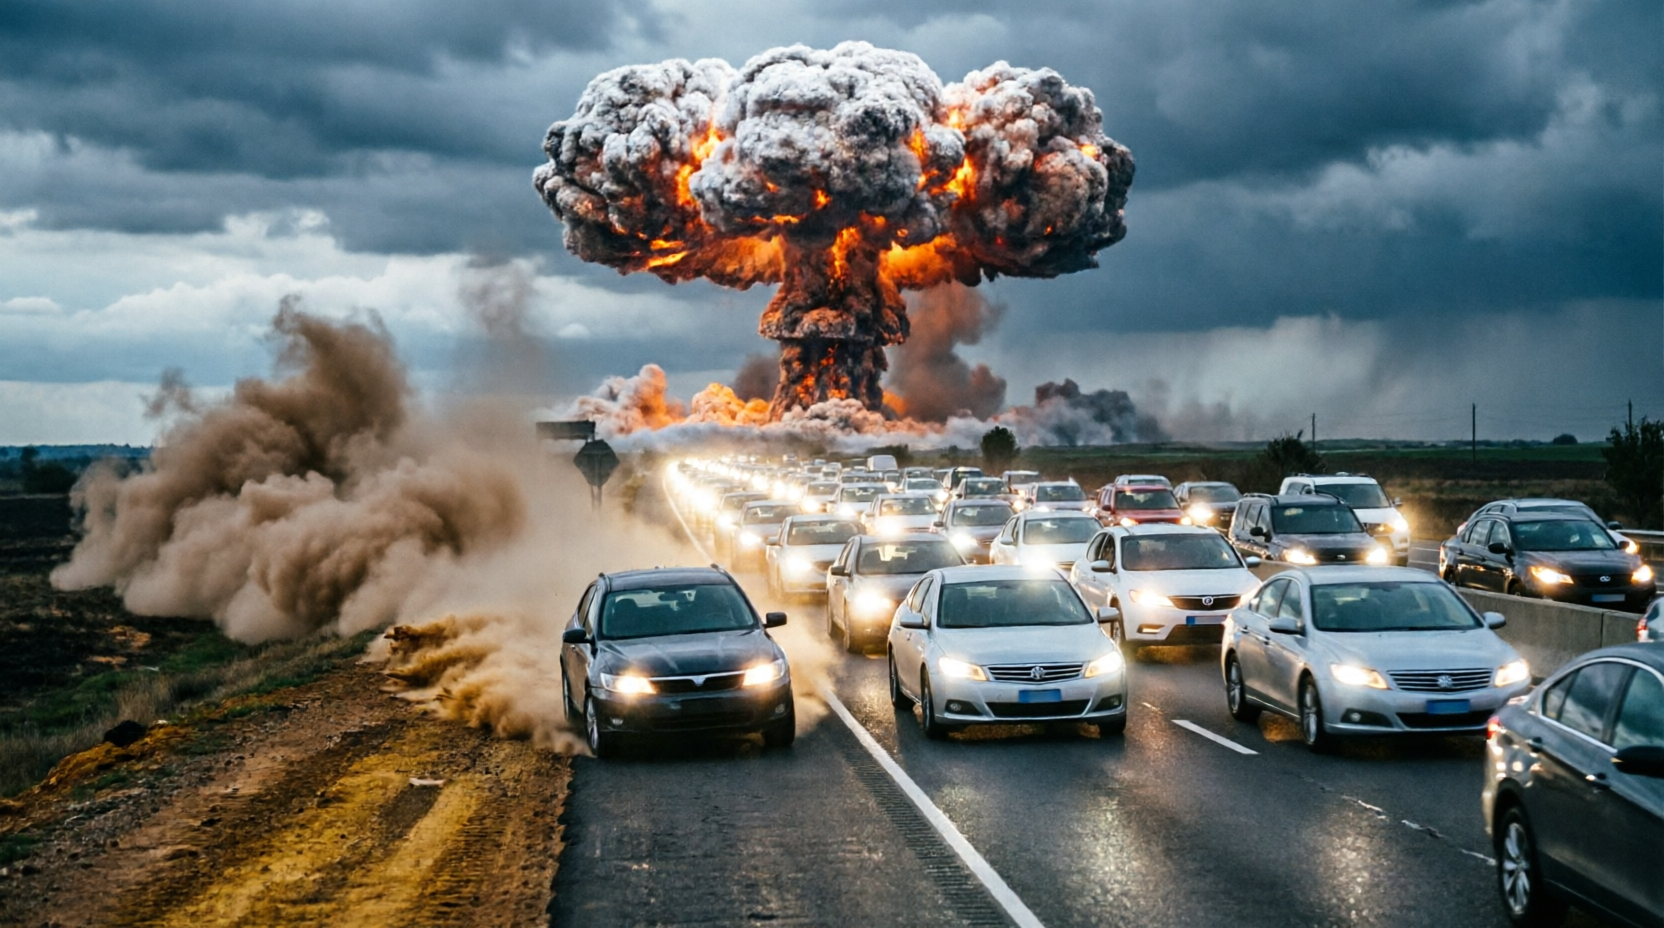
\includegraphics[height=.7\paperheight]{Pics/bang.png}
\end{frame}


\begin{frame}
	\frametitle{Быстрого решения нет}
	\centering
	
\includegraphics[height=.7\paperheight]{Pics/Death.png}
\end{frame}

\section{Мертвые дороги}

\begin{frame}
	\frametitle{Жизнь после\dots}
	\centering
	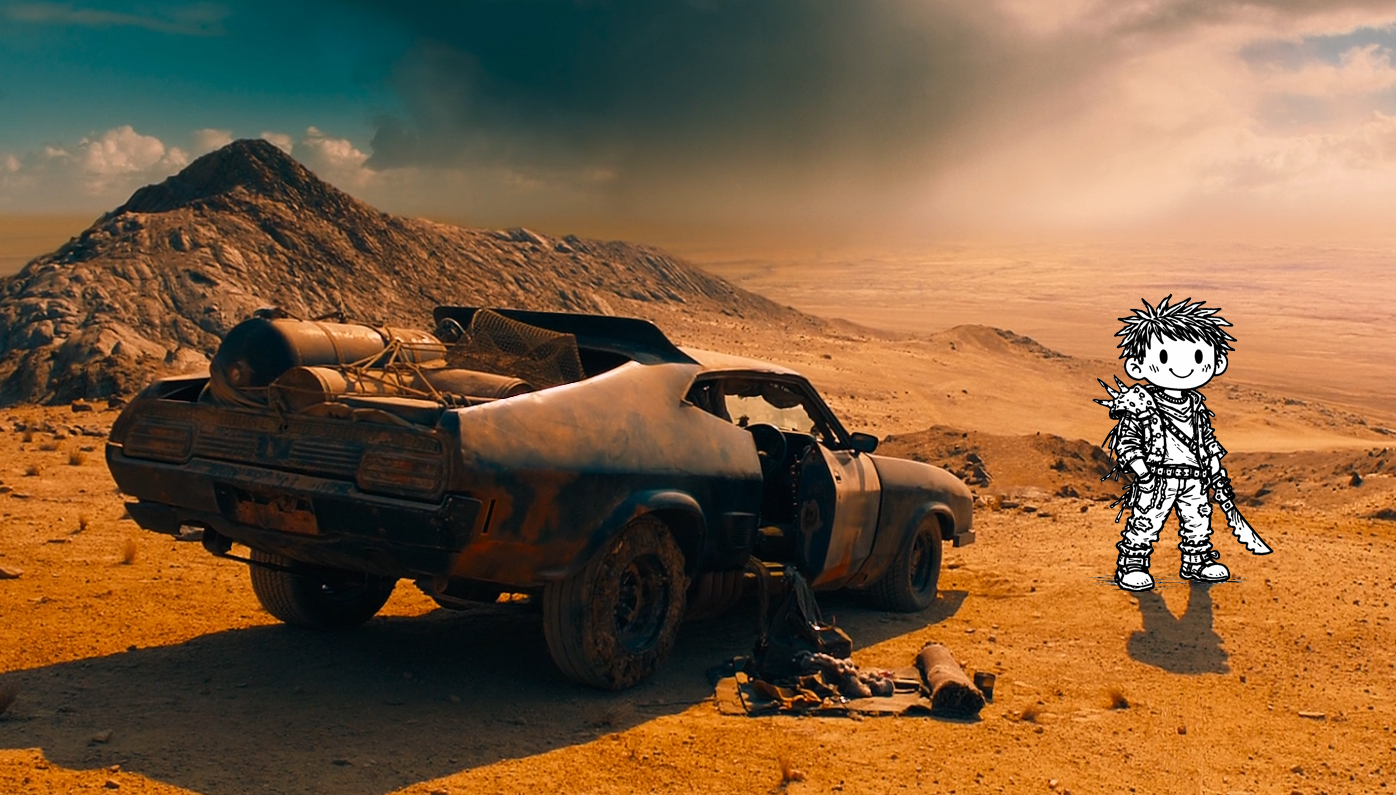
\includegraphics[height=.7\paperheight]{Pics/Max.png}
\end{frame}

\begin{frame}
	\frametitle{Жизнь после\dots}
	\begin{columns}
		\column{.5\textwidth}
		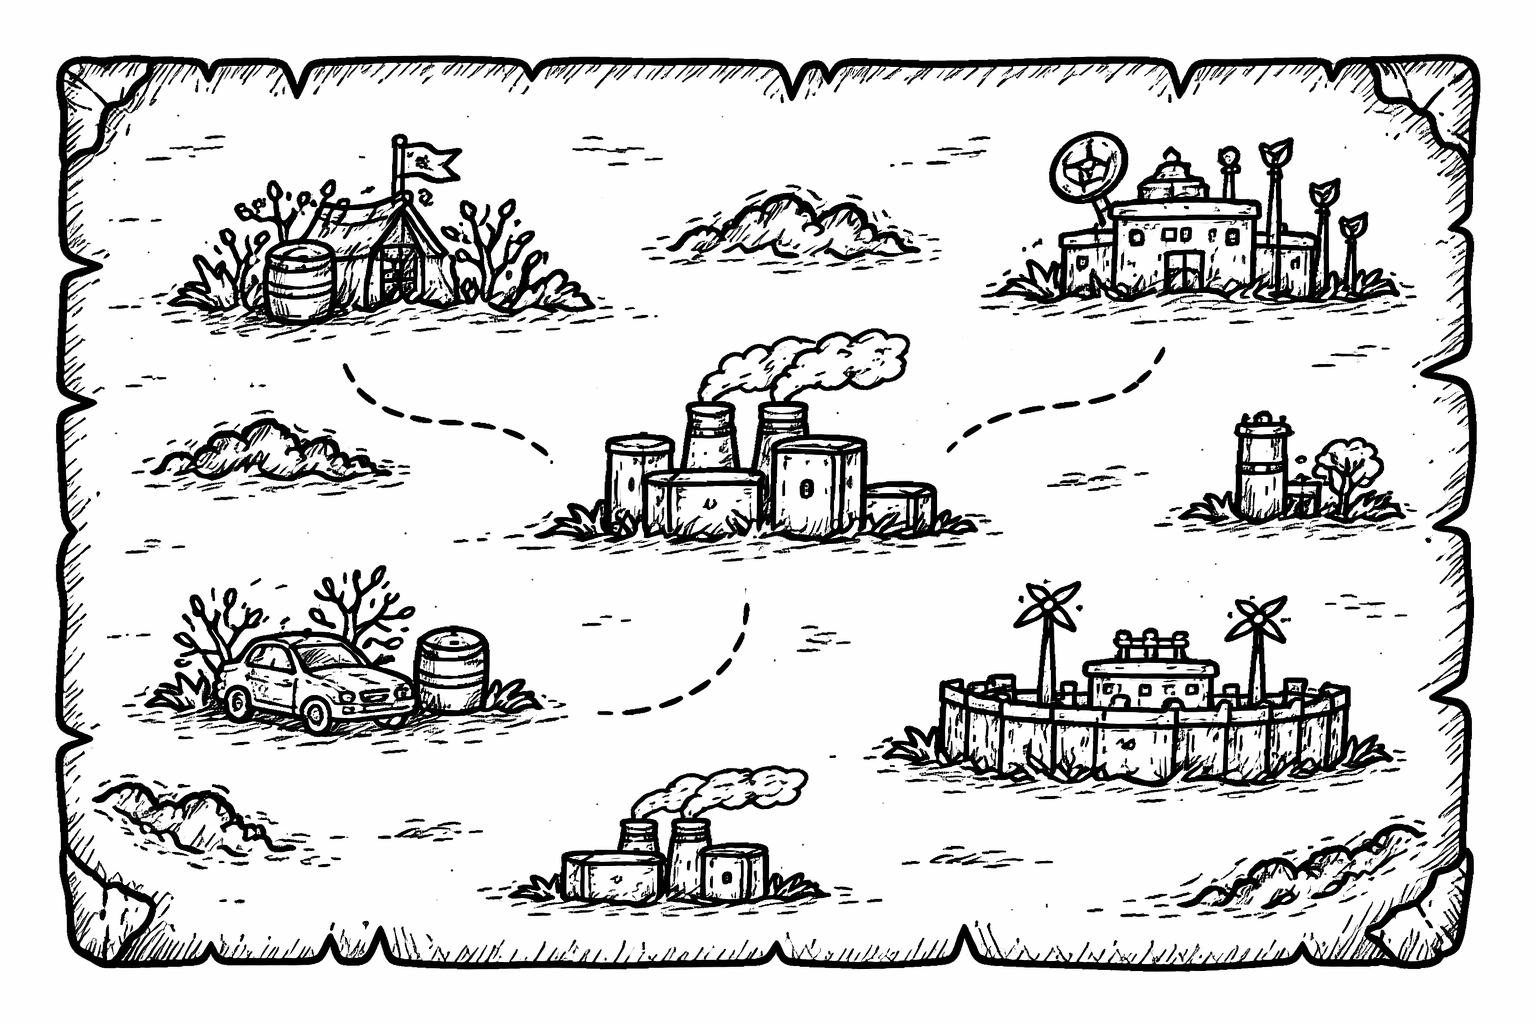
\includegraphics[width=\textwidth]{Pics/postmap.png}

		
\includegraphics[width=.3\textwidth]{Pics/jerrycan.png}
		
\includegraphics[width=.3\textwidth]{Pics/can.png}
		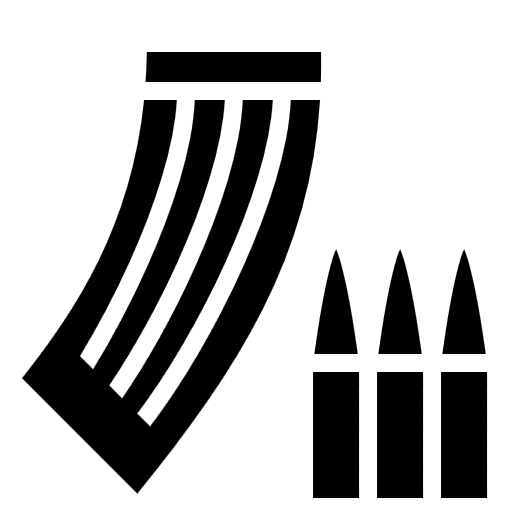
\includegraphics[width=.3\textwidth]{Pics/magazine.png}
		\column{.5\textwidth}
		\begin{block}{Определения}
			\begin{itemize}
				\item Функции ресурса $r_i(e)\colon E\rightarrow \mathbb{R}$;
				\item Величины ограничений ресурса $R_i$;
				\item Траты пути $r_i(P)=\sum\limits_{e\in P}r_i(e)$;
				\item Путь $P$ -- допустимый, если $r_i(P)\leq R_i$.
			\end{itemize}
		\end{block}
	\end{columns}
\end{frame}

\begin{frame}
	\frametitle{Жизнь после\dots}
	\begin{block}{Задача Resource Constrained Shortest Path (RCSP)}
    \textbf{Заданы:} граф $G=(V,E)$, на дугах которого определены положительные вещественнозначные функции $w(e)$, $r_i(e)$, величины $R_i$, $i=1,\dots,l$, и $(s,d)$-запрос.\\
    \textbf{Требуется:} найти в $G=(V,E)$ оптимальный $(s,d)$-маршрут.
  \end{block}
  \begin{columns}
	\column{.45\textwidth}
	\begin{tikzpicture}[scale=0.75,
      ->,    > = stealth',
     shorten > = 1pt,auto,
  node distance = 3cm,
    decoration = {snake,   % <-- added
                  pre length=3pt,post length=7pt,% <-- for better looking of arrow,
                  },
                  ]
      \tikzstyle{v}=[circle,draw, fill=white!20]
      \node[v] (x) {$x$};
      \path (x) + (7,0) node [v] (z) {$z$};
      \path (x) + (3.5,-2) node [v] (y) {$y$};
          \path (x) + (3.5,2) node [v] (v) {$v$};
      \path[draw=blue, thick, ->] (x) -- node[below,sloped] {$w=2, r=3$} (y);
      \path[draw=red, thick, ->] (x) -- node[above,sloped] {$w=2, r=10$} (z);
      \path[draw=blue, thick, ->] (y) -- node[below,sloped] {$w=2, r=2$} (z);
          \path[draw, thick, ->] (x) -- node[above,sloped] {$w=5, r=1$} (v);
          \path[draw, thick, ->] (v) -- node[above,sloped] {$w=2, r=1$} (z);
    \end{tikzpicture}
	\column{.55\textwidth}
	\begin{tabular}{p{0.1\textwidth}p{0.85\textwidth}}
    \setlength\extrarowheight{10pt}
    \tikz\draw[red, thick, -Latex] (0,0) -- (1,0); & Путь $P=\{x,z\}$, $w(P) = 2$, 
	
	$r(P) = 10 \not\leq 5$ (недопустимый)\\\hline
    \tikz\draw[thick, -Latex] (0,0) -- (1,0); & Путь $P=\{x,v,z\}$, $w(P) = 7$, 
	
	$r(P) = 2 \leq 5$ (допустимый)\\\hline
    \tikz\draw[blue, thick, -Latex] (0,0) -- (1,0); & Путь $P=\{x,y,z\}$, $w(P) = 4$, 
	
	$r(P) = 5 \leq 5$ (оптимальный)\\
    \end{tabular}
  \end{columns}
\end{frame}

\begin{frame}
	\frametitle{Чем решать?}
	\begin{block}{Алгоритм Йена}
		Алгоритм находит точное решение путем перебора $k$-кратчайших путей, до тех пор пока не будет найден допустимый путь.

		\begin{itemize}
			\item[$+$] Надежный и находит точное решение
			\item[$-$] Очень долгий $\mathcal{O}\big(k\cdot n\cdot (m + n\log n)\big)$
		\end{itemize}
	\end{block}
	\pause
		\begin{block}{Приближенные алгоритмы}
			\begin{tabular}{p{.25\textwidth}p{.65\textwidth}}
				\texttt{RevTree} & Приближенное решение, зависящее от весов графа.
				
				Сложность $\mathcal{O}(n^2)$.
				\\\hline
				\texttt{Hassin's FPTAS} & Находит решение путем определения верхней и нижней оценок точного решения.

				Сложность $\mathcal{O}(\log\log(U/L)\cdot(n^3(1/\varepsilon + \log\log(U/L))))$.\\
			\end{tabular}
		\end{block}

\end{frame}


\begin{frame}
	\frametitle{Вперед в пустошь}
	\centering
	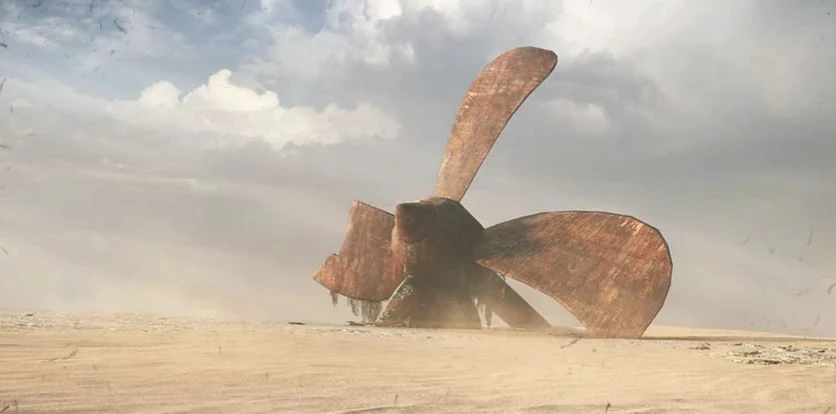
\includegraphics[height=.7\paperheight]{Pics/White.png}
\end{frame}

\begin{frame}
	\frametitle{Вперед в пустошь}
	\begin{block}{Задача канадского путешественника}
		\begin{tabular}{>{\bfseries}rp{.85\textwidth}}
			Дано: & граф-карта $G=(V,E)$, реальный граф $H=(V,E')$, где $E'\subseteq E$, стартовая и целевая вершины $s$ и $d$.\\
			Вопрос: & существует ли такая стратегия $S$ прохождения графа, вес пути в которой будет не более чем в $q$ раз превосходить оптимальное значение кратчайшего пути в $H$.\\
		\end{tabular}
	\end{block}
	\pause
	Задача относится к классу $PSPACE$ и при этом является $\sharp P$-сложной.
\end{frame}

\begin{frame}
	\frametitle{Вперед в пустошь}
	\centering
	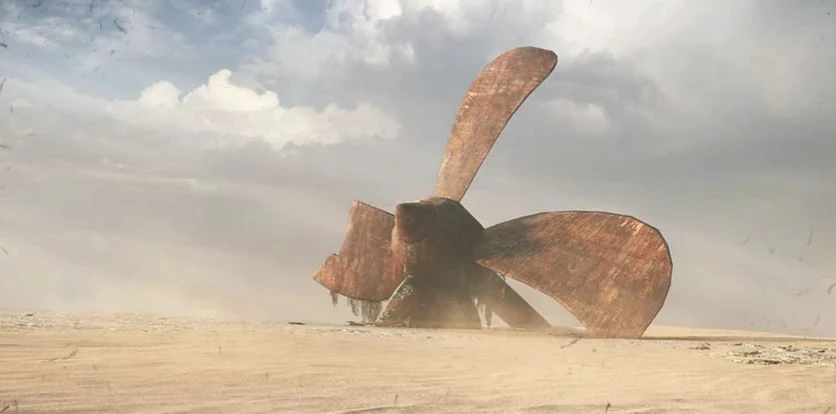
\includegraphics[height=.7\paperheight]{Pics/White.png}
\end{frame}

\section{Киберпространство}
\begin{frame}
	\frametitle{Киберпространство}
	\centering
	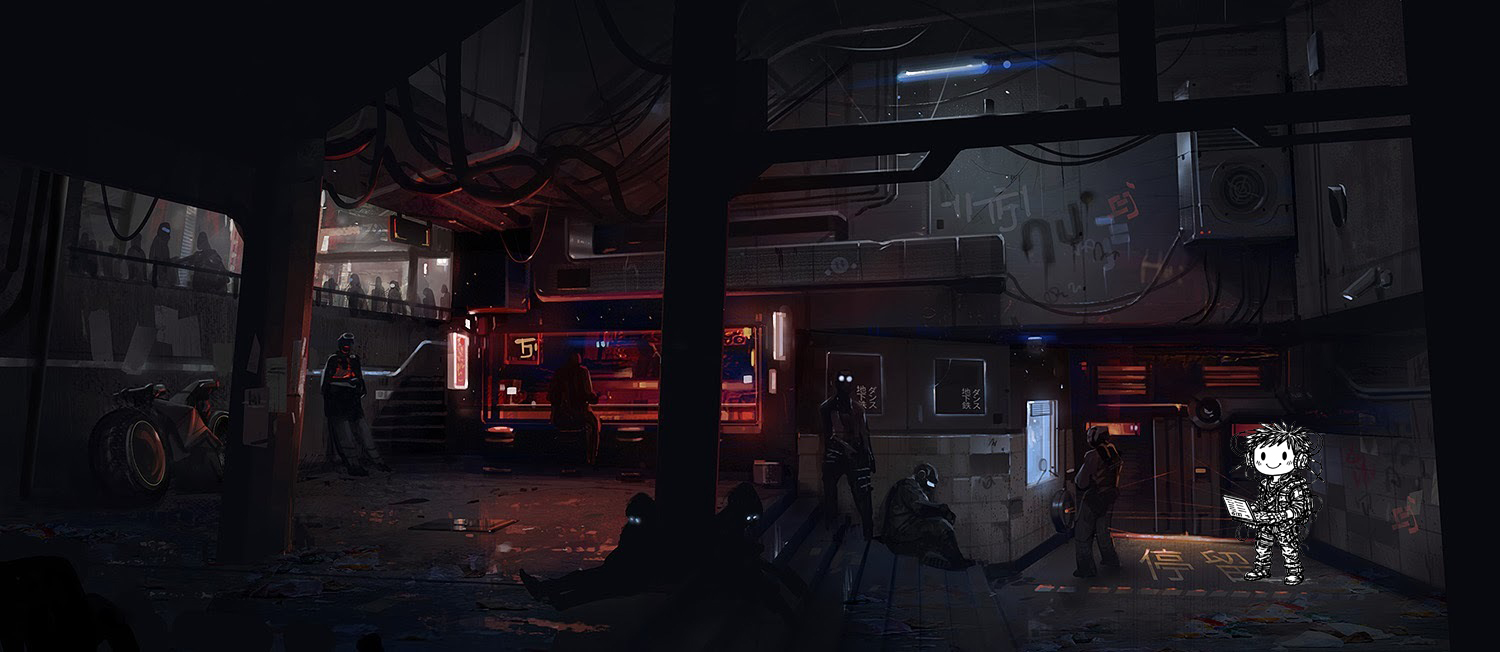
\includegraphics[height=.7\paperheight]{Pics/neucomancer.jpg}
\end{frame}

\begin{frame}
	\frametitle{Киберпространство}
\begin{block}{Задача Multi-Constrained Path (MCP)}
    \textbf{Заданы:} граф $G=(V,E)$, на дугах которого определены положительные вещественнозначные функции $r_i(e)$, величины $R_i$, $i=1,\dots,l$, и $(s,d)$-запрос.\\
    \textbf{Требуется:} найти в $G=(V,E)$ допустимый $(s,d)$-маршрут.
  \end{block}
\end{frame}

\begin{frame}
	\frametitle{Как решать?}
\begin{block}{Случай двух ограничений}
	Алгоритм \texttt{P+RT} основан на построении в процессе работы <<мостов>>, которые создают допустимые подпути. Затем на основе данных мостов алгоритм восстанавливает топологию исходного графа и находит аппроксимацию допустимого пути.

	Алгоритм является $(3\cdot(1+\varepsilon),2)$-приближенным.

	Работает за время $\mathcal{O}\big(mn(1/\varepsilon + \log n)\big)$.
\end{block}
\pause
\begin{block}{Случай произвольного числа ограничений}
	Алгоритм $(1+\varepsilon)(l-1)$-\texttt{Approx} основан на построении вспомогательного графа, в котором выполняется поиск приближенного решения, согласно вычисленным верхним и нижним оценкам допустимого решения.

	Алгоритм находит $(1+\varepsilon)(l-1)$-приближение.

	Работает за время $\mathcal{O}\big(mn\log\log\log n + m(n/\varepsilon)^{l-1}\big)$.
\end{block}
\end{frame}

\begin{frame}
	\frametitle{Слияние ИскИнов}
	\centering
	\includegraphics[height=.7\paperheight]{Pics/Collapse.png}
\end{frame}

\section{Неизвестное}

\begin{frame}
	\frametitle{Расхитители древности}
	\centering
	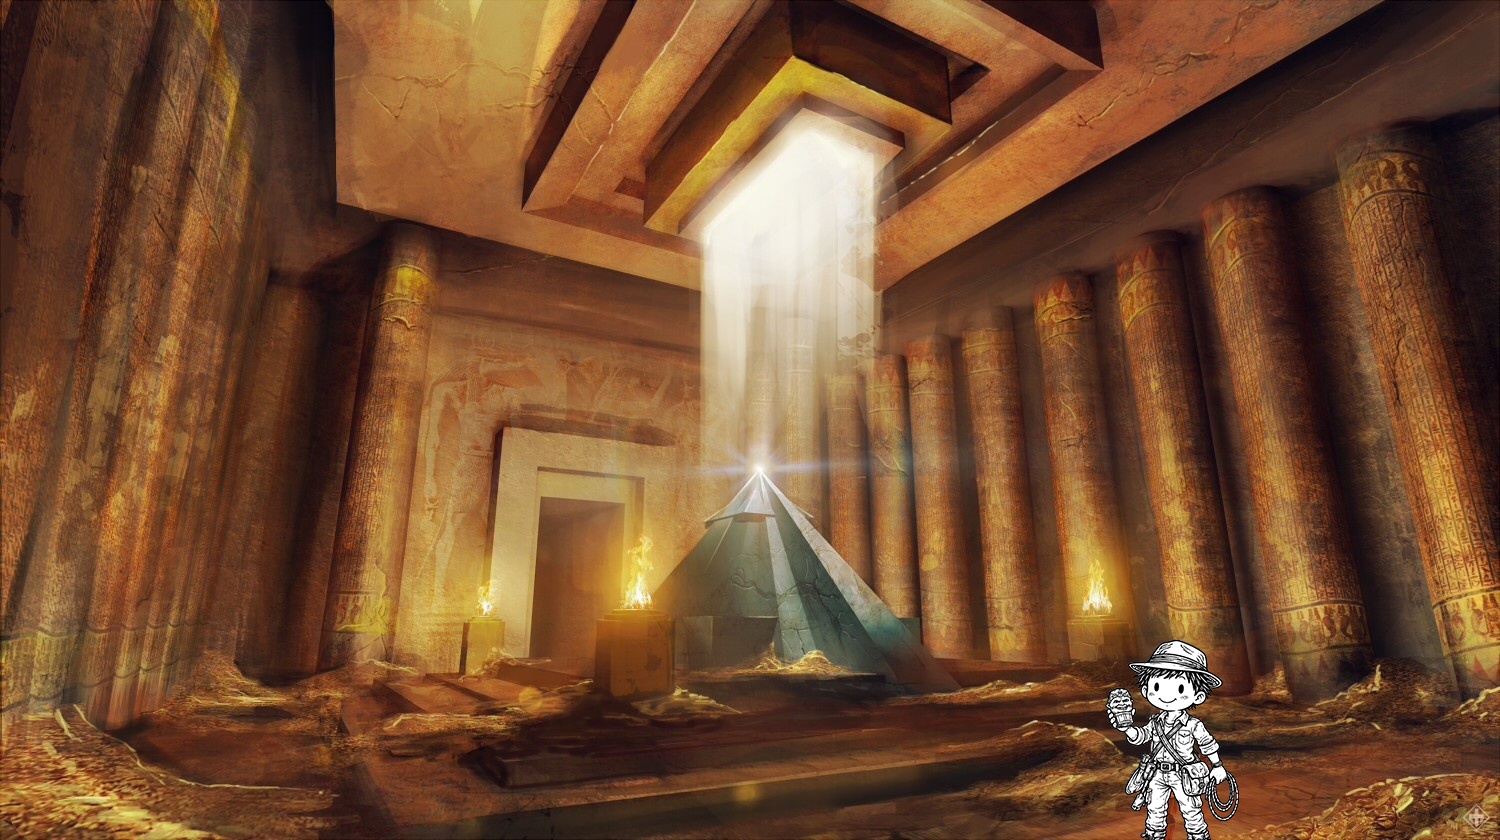
\includegraphics[height=.7\paperheight]{Pics/tomb.png}
\end{frame}

\begin{frame}
	\frametitle{Расхитители древности}
	\centering
	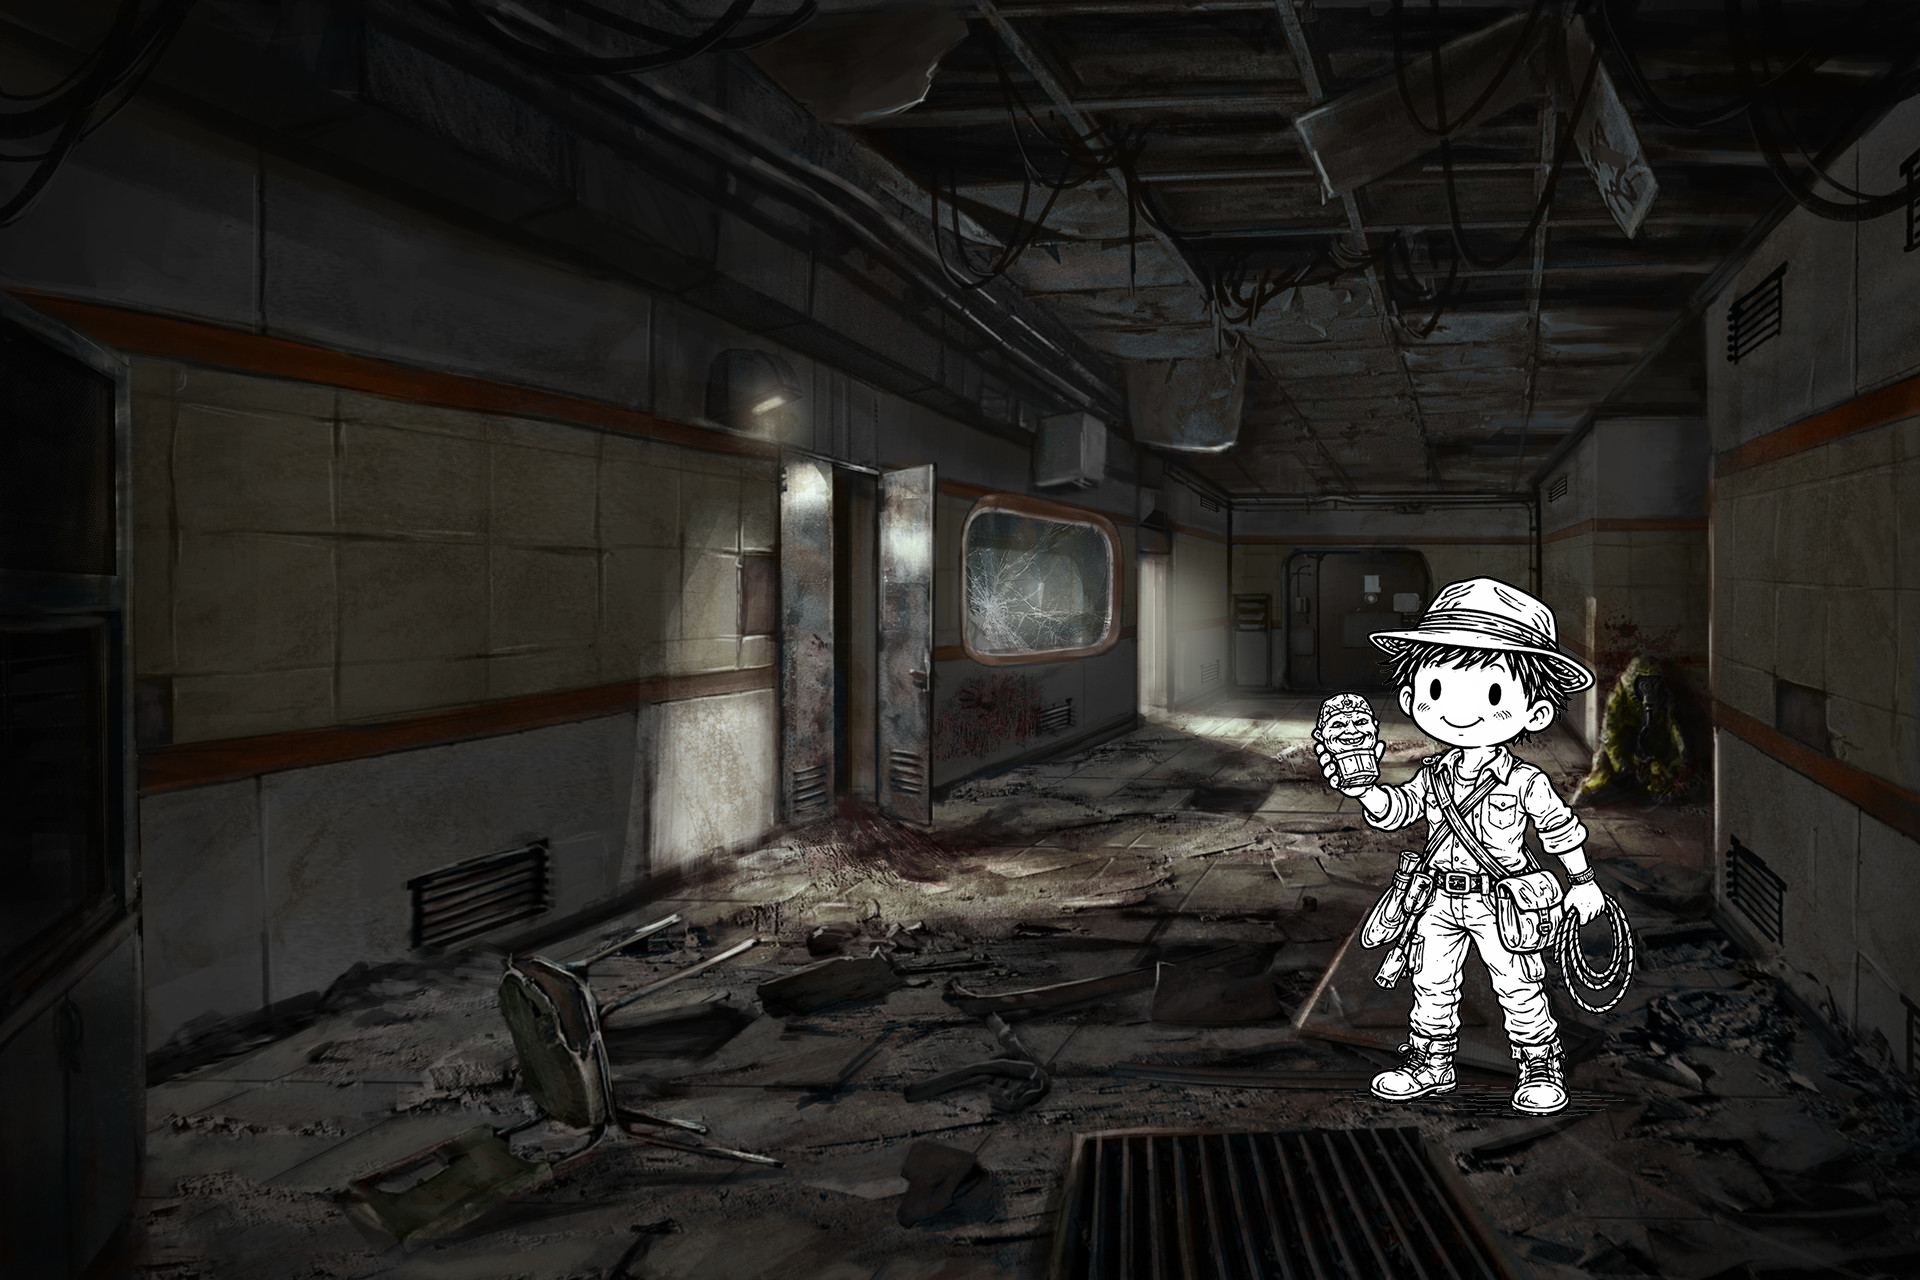
\includegraphics[height=.7\paperheight]{Pics/facility.png}
\end{frame}

\begin{frame}
	\frametitle{Расхитители древности}
	\begin{block}{Определения}
		\begin{itemize}
			\item Функция разрушения $f\colon V\rightarrow E$.
			\item Саморазрушающийся граф $(G,f)$, где $G=(V,E)$ -- граф и $f$ -- функция разрушения, заданная на вершинах.
			\item Маршрутом назовем последовательность вершин и ребер $(v_1,e_1,v_2,e_2,\dots,e_{k-1},v_k)$, где $v_i$ и $v_j$ могут совпадать при $i\neq j$.
			\item Путь или маршрут в графе $G$ называется $f$-согласованным, если для всех $j\leq i$ выполняется условие $e_i\notin f(v_j)$.
		\end{itemize}
	\end{block}
\end{frame}

\begin{frame}
	\frametitle{Расхитители древности}
	\begin{block}{Задача о пути в саморазрушающемся графе}
		\begin{tabular}{>{\bfseries}rp{.85\textwidth}}
			Дано: & функция разрушения $f$, саморазрушающийся граф $(G,f)$, стартовая вершина $s$ и целевая вершина $d$.\\
			Вопрос: & существует ли в саморазрушающемся графе $(G,f)$ $f$-согласованный $(s,d)$-путь?
		\end{tabular}
	\end{block}
\pause
\begin{center}
	\begin{overprint}
		\onslide<2>
		\begin{tikzpicture}[every node/.style={draw,circle,fill=black},node distance = .5cm]
		\node[pin=90:$s$] (a) {};
		\node[fill= red,above right = of a] (a1) {};
		\node[fill= blue,below right = of a] (a2) {};
		\node[above right = of a2] (a3) {};
		\node[right = of a3] (b) {};
		\node[fill= green,above right = of b] (b1) {};
		\node[fill= orange,below right = of b] (b2) {};
		\node[above right = of b2] (b3) {};
		\node[right = of b3] (c) {};
		\node[fill= violet,above right = of c] (c1) {};
		\node[fill= pink,below right = of c] (c2) {};
		\node[above right = of c2] (c3) {};
		\node[above right = .2cm and .5cm of c3] (d1) {};
		\node[below = of d1] (d2) {};
		\node[right = of d1] (d3) {};
		\node[right = of d2] (d4) {};
		\node[right = of d3] (d5) {};
		\node[right = of d4] (d6) {};
		\node[right = of d5] (e1) {};
		\node[right = of d6] (e2) {};
		\node[right = of e1] (e3) {};
		\node[right = of e2] (e4) {};
		\node[right = of e3] (e5) {};
		\node[right = of e4] (e6) {};
		\node[right = of e5] (f1) {};
		\node[right = of e6] (f2) {};
		\node[right = of f1] (f3) {};
		\node[right = of f2] (f4) {};
		\node[right = of f3] (f5) {};
		\node[right = of f4,pin=45:$d$] (f6) {};
		\draw (a) -- (a1) -- (a3) -- (b) -- (b1) -- (b3) -- (c) -- (c1) -- (c3) -- (d1);
		\draw (a) -- (a2) -- (a3);
		\draw (b) -- (b2) -- (b3);
		\draw (c) -- (c2) -- (c3);
		\draw (d1) -- (d3) -- (d5);
		\draw (d2) -- (d4) -- (d6)--(e1);
		\draw (e1) -- (e3) -- (e5);
		\draw (e2) -- (e4) -- (e6)--(f1);
		\draw (f1) -- (f3) -- (f5);
		\draw (f2) -- (f4) -- (f6);
		\draw[very thick,blue] (d1) -- (d2);
		\draw[very thick,green] (d3) -- (d4);
		\draw[very thick,violet] (d5) -- (d6);
		\draw[very thick,red] (e1) -- (e2);
		\draw[very thick,orange] (e3) -- (e4);
		\draw[very thick,violet] (e5) -- (e6);
		\draw[very thick,red] (f1) -- (f2);
		\draw[very thick,orange] (f3) -- (f4);
		\draw[very thick,pink] (f5) -- (f6);
	\end{tikzpicture}
	\onslide<3>
	\begin{tikzpicture}[every node/.style={circle,fill=black},node distance = .5cm]
		\node[draw, pin=90:$s$] (a) {};
		\node[right=.1cm of a,fill=none] {$x$};
		\node[draw, fill= red,above right = of a] (a1) {};		
		\node[draw, fill= blue,below right = of a] (a2) {};
		\node[draw, above right = of a2] (a3) {};
		\node[draw, right = of a3] (b) {};
		\node[right=.1cm of b,fill=none] {$y$};
		\node[draw, fill= green,above right = of b] (b1) {};
		\node[draw, fill= orange,below right = of b] (b2) {};
		\node[draw, above right = of b2] (b3) {};
		\node[draw, right = of b3] (c) {};
		\node[right=.1cm of c,fill=none] {$z$};
		\node[draw, fill= violet,above right = of c] (c1) {};
		\node[draw, fill= pink,below right = of c] (c2) {};
		\node[draw, above right = of c2] (c3) {};

		\node[inner sep =-.1cm, above=.1cm of a1,fill=none] {\texttt{True}};
		\node[inner sep =-.1cm, above=.1cm of b1,fill=none] {\texttt{True}};
		\node[inner sep =-.1cm, above=.1cm of c1,fill=none] {\texttt{True}};
		\node[inner sep =-.1cm, below=.1cm of a2,fill=none] {\texttt{False}};
		\node[inner sep =-.1cm, below=.1cm of b2,fill=none] {\texttt{False}};
		\node[inner sep =-.1cm, below=.1cm of c2,fill=none] {\texttt{False}};		

		\node[draw, above right = .2cm and .5cm of c3] (d1) {};
		\node[draw, below = of d1] (d2) {};
		\node[draw, right = of d1] (d3) {};
		\node[draw, right = of d2] (d4) {};
		\node[draw, right = of d3] (d5) {};
		\node[draw, right = of d4] (d6) {};
		\node[draw, right = of d5] (e1) {};
		\node[draw, right = of d6] (e2) {};
		\node[draw, right = of e1] (e3) {};
		\node[draw, right = of e2] (e4) {};
		\node[draw, right = of e3] (e5) {};
		\node[draw, right = of e4] (e6) {};
		\node[draw, right = of e5] (f1) {};
		\node[draw, right = of e6] (f2) {};
		\node[draw, right = of f1] (f3) {};
		\node[draw, right = of f2] (f4) {};
		\node[draw, right = of f3] (f5) {};
		\node[draw, right = of f4,pin=45:$d$] (f6) {};
		\draw (a) -- (a1) -- (a3) -- (b) -- (b1) -- (b3) -- (c) -- (c1) -- (c3) -- (d1);
		\draw (a) -- (a2) -- (a3);
		\draw (b) -- (b2) -- (b3);
		\draw (c) -- (c2) -- (c3);
		\draw (d1) -- (d3) -- (d5);
		\draw (d2) -- (d4) -- (d6)--(e1);
		\draw (e1) -- (e3) -- (e5);
		\draw (e2) -- (e4) -- (e6)--(f1);
		\draw (f1) -- (f3) -- (f5);
		\draw (f2) -- (f4) -- (f6);
		\draw[very thick,blue] (d1) -- (d2);
		\draw[very thick,green] (d3) -- (d4);
		\draw[very thick,violet] (d5) -- (d6);
		\draw[very thick,red] (e1) -- (e2);
		\draw[very thick,orange] (e3) -- (e4);
		\draw[very thick,violet] (e5) -- (e6);
		\draw[very thick,red] (f1) -- (f2);
		\draw[very thick,orange] (f3) -- (f4);
		\draw[very thick,pink] (f5) -- (f6);

		\draw [decorate, decoration = {brace}] (d1.north west)+(0,.1) -- ($(d5.north east)+(0,.1)$) node[above,midway,fill=none,rectangle] {Скобка 1};
		\draw [decorate, decoration = {brace}] (e1.north west)+(0,.1) -- ($(e5.north east)+(0,.1)$) node[above,midway,fill=none,rectangle] {Скобка 2};
		\draw [decorate, decoration = {brace}] (f1.north west)+(0,.1) -- ($(f5.north east)+(0,.1)$) node[above,midway,fill=none,rectangle] {Скобка 3};

	\end{tikzpicture}
	\onslide<4>
	\begin{tikzpicture}[every node/.style={circle,fill=black},node distance = .5cm]
		\node[draw, pin=90:$s$] (a) {};
		\node[right=.1cm of a,fill=none] {$x$};
		\node[draw, fill= red,above right = of a] (a1) {};		
		\node[draw, fill= blue,below right = of a] (a2) {};
		\node[draw, above right = of a2] (a3) {};
		\node[draw, right = of a3] (b) {};
		\node[right=.1cm of b,fill=none] {$y$};
		\node[draw, fill= green,above right = of b] (b1) {};
		\node[draw, fill= orange,below right = of b] (b2) {};
		\node[draw, above right = of b2] (b3) {};
		\node[draw, right = of b3] (c) {};
		\node[right=.1cm of c,fill=none] {$z$};
		\node[draw, fill= violet,above right = of c] (c1) {};
		\node[draw, fill= pink,below right = of c] (c2) {};
		\node[draw, above right = of c2] (c3) {};

		\node[inner sep =-.1cm, above=.1cm of a1,fill=none] {\texttt{True}};
		\node[inner sep =-.1cm, above=.1cm of b1,fill=none] {\texttt{True}};
		\node[inner sep =-.1cm, above=.1cm of c1,fill=none] {\texttt{True}};
		\node[inner sep =-.1cm, below=.1cm of a2,fill=none] {\texttt{False}};
		\node[inner sep =-.1cm, below=.1cm of b2,fill=none] {\texttt{False}};
		\node[inner sep =-.1cm, below=.1cm of c2,fill=none] {\texttt{False}};		

		\node[draw, above right = .2cm and .5cm of c3] (d1) {};
		\node[draw, below = of d1] (d2) {};
		\node[draw, right = of d1] (d3) {};
		\node[draw, right = of d2] (d4) {};
		\node[draw, right = of d3] (d5) {};
		\node[draw, right = of d4] (d6) {};
		\node[draw, right = of d5] (e1) {};
		\node[draw, right = of d6] (e2) {};
		\node[draw, right = of e1] (e3) {};
		\node[draw, right = of e2] (e4) {};
		\node[draw, right = of e3] (e5) {};
		\node[draw, right = of e4] (e6) {};
		\node[draw, right = of e5] (f1) {};
		\node[draw, right = of e6] (f2) {};
		\node[draw, right = of f1] (f3) {};
		\node[draw, right = of f2] (f4) {};
		\node[draw, right = of f3] (f5) {};
		\node[draw, right = of f4,pin=45:$d$] (f6) {};
		\draw (a) -- (a1) -- (a3) -- (b) -- (b1) -- (b3) -- (c) -- (c1) -- (c3) -- (d1);
		\draw (a) -- (a2) -- (a3);
		\draw (b) -- (b2) -- (b3);
		\draw (c) -- (c2) -- (c3);
		\draw (d1) -- (d3) -- (d5);
		\draw (d2) -- (d4) -- (d6)--(e1);
		\draw (e1) -- (e3) -- (e5);
		\draw (e2) -- (e4) -- (e6)--(f1);
		\draw (f1) -- (f3) -- (f5);
		\draw (f2) -- (f4) -- (f6);
		\draw[very thick,blue] (d1) -- (d2);
		\draw[very thick,green] (d3) -- (d4);
		\draw[very thick,violet] (d5) -- (d6);
		\draw[very thick,red] (e1) -- (e2);
		\draw[very thick,orange] (e3) -- (e4);
		\draw[very thick,violet] (e5) -- (e6);
		\draw[very thick,red] (f1) -- (f2);
		\draw[very thick,orange] (f3) -- (f4);
		\draw[very thick,pink] (f5) -- (f6);

		\draw [decorate, decoration = {brace}] (d1.north west)+(0,.1) -- ($(d5.north east)+(0,.1)$) node[above,midway,fill=none,rectangle] {Скобка 1};
		\draw [decorate, decoration = {brace}] (e1.north west)+(0,.1) -- ($(e5.north east)+(0,.1)$) node[above,midway,fill=none,rectangle] {Скобка 2};
		\draw [decorate, decoration = {brace}] (f1.north west)+(0,.1) -- ($(f5.north east)+(0,.1)$) node[above,midway,fill=none,rectangle] {Скобка 3};

	\end{tikzpicture}
	\vspace*{-.5cm}
	$$\varphi = (x\vee\bar{y}\vee\bar{z})\wedge(\bar{x}\vee y\vee \bar{z})\wedge(\bar{x}\vee y\vee z)$$
	\end{overprint}		
\end{center}		
\end{frame}

\begin{frame}
	\LARGE\bfseries\centering Благодарю за внимание!
\end{frame}
\end{document}
